\section{Resource Sharing And Binding Methods}

% sharing def
% binding def
% problem - The Spatial Domain: Binding 

% sharing and binding method 

% Non-Hierarchical Sequencing Graphs 
% Hierarchical Sequencing Graphs 

% Register Sharing 
% Multi-Port Memory Binding 
% Bus Sharing and Binding 
% UnconsIrGned Minimum-Area Binding* 
% Performance-ConsIrained and Performance-Directed Binding*

In this section one of the most important processes in synthesizing an architecture model will be discussed which is resource sharing and binding. We assume here scheduled sequencing graph and non-hierarchical sequencing graph only. Before going through the methods used to solve resource sharing and binding problem, the definition of them should be comprehended as follows \cite{main}:

\begin{itemize}
    \item Resource sharing : A resource is assigned to more than one operation
    \item Binding : Mapping of an operation to a physical resource, $\beta : V \xrightarrow{} R * Z^{+}$, where $\beta(v_{i})$, where $\beta(v_{i})=(t,r)$ denotes that the operation corresponding to $v_{i} \in V$, with type $\tau(c_{i}) = t$, is implemented by the $r^{th}$ instance of resource type $t \in R$ for each $i = 1,2,...,n_{ops}$
\end{itemize}

If more than one operation with the same type are used, like in our sample model, resource sharing can be implemented as long as the operations are not concurrent, means that $ E=\{(v_{i},v_{j})|\tau(v_{i}=v_{j} $ and $ ((t_{i}=d_{i} \leq t_{j}) $ or $ t_{j}=d{j} \leq t_{i})),i,j=1,...,n_{ops}\}$. The operation is \textit{compatible} if those conditions are met \cite{main}. The need of sharing is to reduce the area of a circuit. Some circuit specification already have area constraint that need to be followed, means that resource sharing need to be applied. It is also possible that the binding constraint already specified in a circuit specification. To reduce the complexity, our model circuit does not have binding constraint, but area constraint maybe applied and will be explained later. Many methods have been proposed to help designer to decide which operations are compatible and how many resources should be used. Resource sharing implicitly describe the binding of an operation to a specific resource. That means every method used to solve resource sharing problem involve binding problem. 

Next, we will discuss the methods used to determine the compatibility of operation for sharing. First, for the sake of simplicity, we assume that our model circuit is a resource dominated circuit, and then we will assume our model circuit is a general circuit to help the reader understand the method. 

\subsection{Compatibility Graph}

 One of the method to analyse the compatibility of operation for sharing is using Compatibility graph. Compatibility graph, $G_{+}(V,E)$ is a graph whose vertex set  $  V = \{v_{i}, i = 1,2,..., n_{ops}\} $ is in one to one correspondence with the operation and whose edge set $ E = \{\{v_{i},v_{j} i,j = 1,2,...,n_{ops}\}$ denotes the compatible operation pairs \cite{main}. This means that the number of distinct components in the graph is at least equal to the number of resource categories. An optimal resource sharing strategy is one that reduces the amount of resources instance required\cite{main}.
 
 According to \cite{main}---``A group of mutually compatible operations corresponds to a subset of vertices that are all mutually connected by edges, i.e., to a clique. Therefore, a minimal set of mutually compatible operations is represented by a maximal clique in the compatibility graph. Since we can associate a resource instance to each clique, the problem is equivalent to partitioning the graph into a minimum number of cliques. Such a number is the clique cover number of $G_{+}(V,E)  $, denoted by $\kappa(G_{+}(V,E)) $"

 Base on our sample model, the compatibility graph can be drawn as in ``Fig. \ref{Compatibility_graph}. Each vertex representing the operation type. We can see that $\{v_{2},v_{6}\} $ and $\{v_{10},v_{11}\} $ are examples of compatible operation.  Examples of cliques are the sub-graphs induced by $\{v_{1},v_{3},v_{7}\}  $,$\{ v_{2},v_{6},v_{8}\} $,$\{ v_{4},v_{5}, v_{10}, v_{11}\}$ $ \{v_{9}\} $. So the clique cover number $ \kappa $ of the graph is 4, corresponding to two multipliers and two ALUs. The edges of a clique are thicker than the other, as shown in ``Fig. \ref{Compatibility_graph}.
 

\begin{figure}[h]
    \centering
    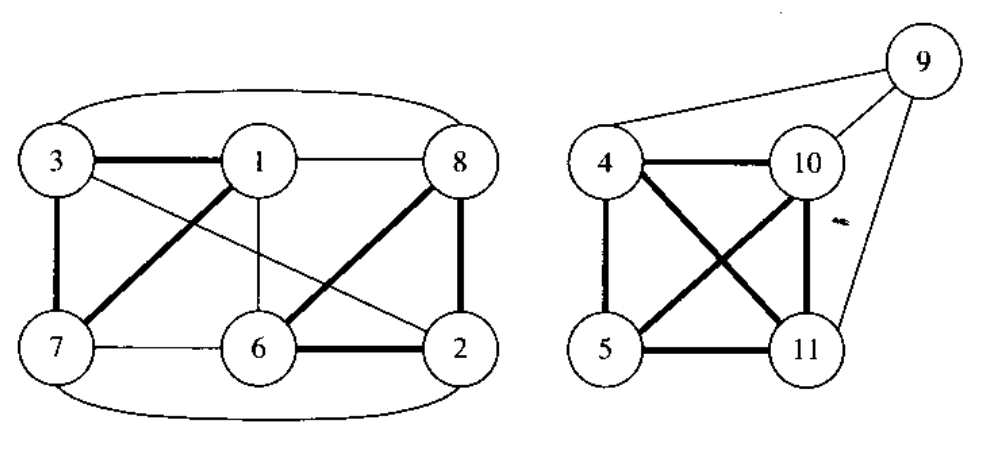
\includegraphics[width=0.4\textwidth]{Compatibility_graph}
    \caption{ Compatibility graph. \cite{main}}
    \label{Compatibility_graph}
\end{figure}

Since the area of a general circuit is not only depends on resource but also involving the area of steering logic and wiring, we need to extend the compatibility graph to help designer estimate area more accurately. To make explanation much simpler, we only focus on the multiplexer, whose  area and propagation delays depend on the number of inputs and wires \cite{main}.

We extend the compatibility graph to a weighted compatibility graph.  Different types of weighted compatibility graphs can be defined \cite{main}. As mentioned before, we can represent the sub-graph as a clique. Cliques may be connected with weight. The cost of allocating the clique to a single resource comprehend the cost of steering logic and wiring components like multiplexers.

A set inclusion cost function can be used to create a weighted compatibility graph model \cite{main}. Each vertex of the compatibility graph in this model is assigned a set of weights known as a cost set. The total cost is the sum of all weights associated with a partition's cliques. The cost-set approach allows us to compute weights on cliques based on vertices' properties. This model may be used to describe the steering logic and wiring area, which are dependent on operation grouping and binding to a shared resource.

Now we consider the operation in ``Fig. \ref{Compatibility_graph}" within the first clique that use multiplier. Assuming that the cost of multiplexing $a$ signal is $area_{mux} = area_{mux}^{ \bigtriangleup}(a-1)$ and is expressed as $area_{M}^{0} = \sum_{i=1}^{a} area_{M}^{i}$, where $area_{mux}^{ \bigtriangleup}=area_{M}^{i}= -area_{M}^{0}$, $1 \leq i \leq a$ \cite{main}.

If we assume each operation with dedicated resource, the overall cost is $(area_{*} + area_{M}^{0}) + \sum_{i=1}^{3} area_{M}^{i}  = 3area_{*}$. If we assume operation $v_{3}$ and $v_{1}$ share the same resource, and $v_{7}$ with dedicated resource, the overall cost is $(area_{*} + area_{M}^{0} +\sum_{i=1}^{3} area_{M}^{i}) + (area_{*},area_{M}^{0},area_{M}^{3})  = 2area_{*} + area_{mux}^{ \bigtriangleup}(2-1)$.

So, we can conclude that this method  could help designer to decide the compatibility of operations under the constrained area. Another technique that based on compatible graph as mention in \cite{main} that purposed by Tseng and Siewiorek is clique partitioning algorithm that constructs cliques from compatible pairs of operations. Means that they utilized edge weights to reflect the intensity of desire for sharing. The edge-weighted compatibility graph is denoted here by $G_{+}(V, E, W)$.

Again, we consider the operation in ``Fig. \ref{Compatibility_graph}". The subgraph's two vertices with the most common neighbours are merged. If the edge is not connected to all the member of the new vertex (clique seed), the edge will be deleted. This process is repeated until no connected edge left. Then the formed clique will be saved on a list.  This process can be illustrated in ``Fig. \ref{Comparibility_graph_mux_2}"

\begin{figure}[h]
    \centering
    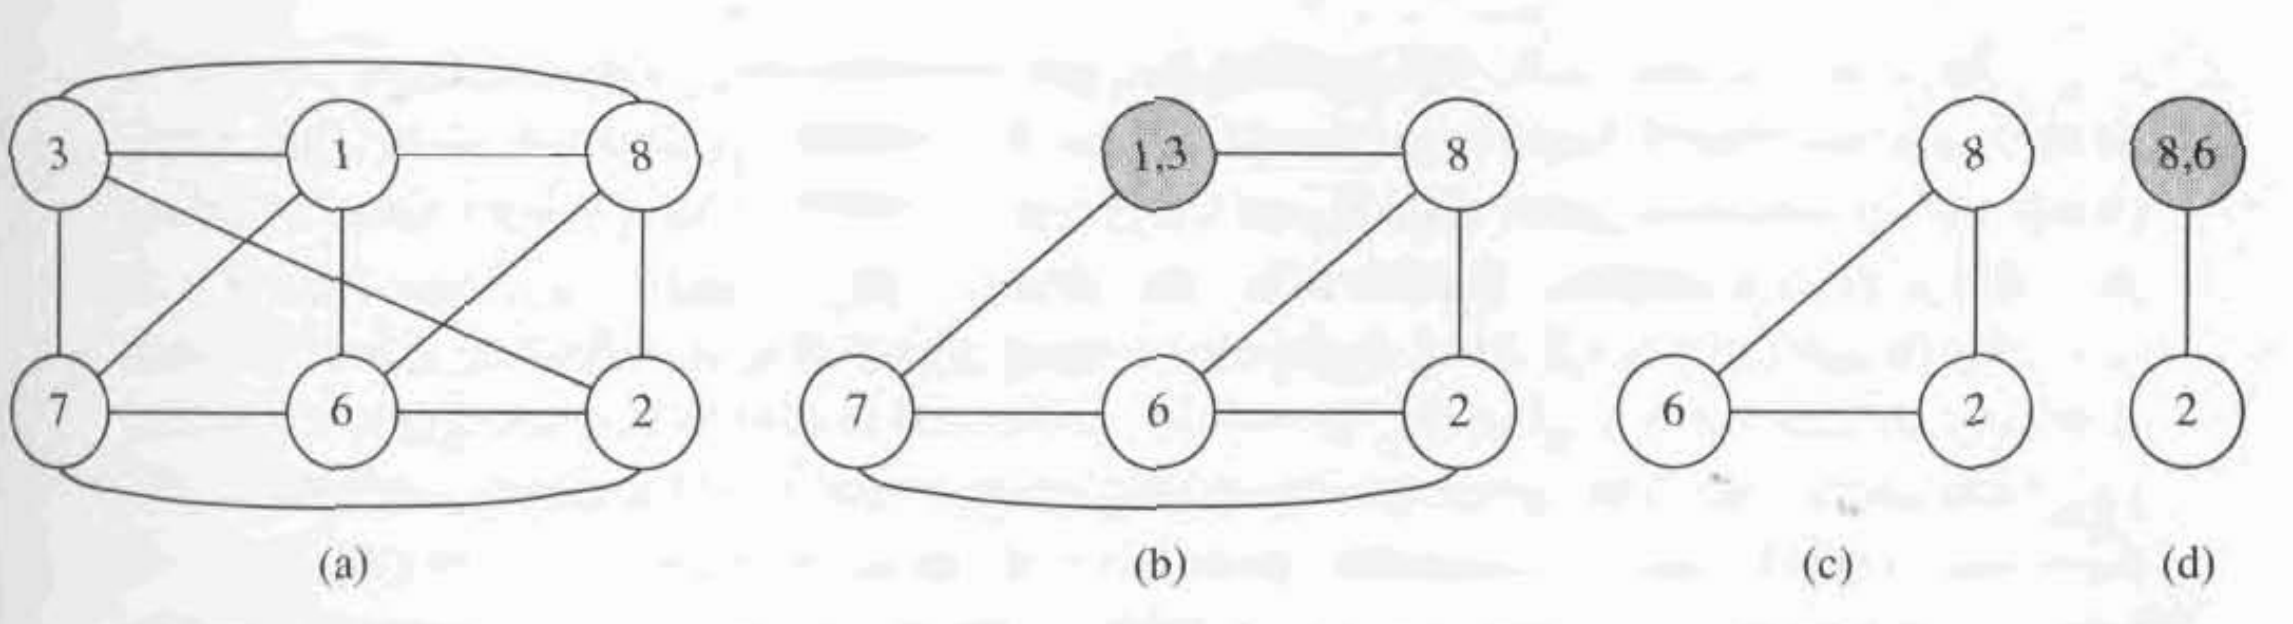
\includegraphics[width=0.5\textwidth]{Comparibility_graph_mux_2}
    \caption{ (a) Compatibility graph for the multiplier type. (b) Reduced compatibility graph with clique seed. (c) Fragment of compatibility graph after one clique has been removed. (d) Reduced fragment with clique seed. \cite{main}}
    \label{Comparibility_graph_mux_2}
\end{figure}

Next, we will go through  another method used to analyse the compatibility of operation for sharing other than compatibility graph, which is conflict graph.


\subsection{Conflict Graph}

Compatibility of operation for sharing can be analysed using Conflict graph. Conflict graph, $G_{-}(V, E)$ is a graph, is a graph whose vertex set $ V = \{ v_{i}, i = 1, 2, ..., n_{ops}\}$ is in one-to-one correspondence with the operations and whose edge set $E = \{\{v_{i},v_{j}\} i, j = 1, 2, ...,n_{ops}\}$ denotes the conflicting operation pairs.Operations have conflict when they are not compatible \cite{main}. Means that the graph is the compliment of the compatibility graph because a subset of vertices that are not linked by edges corresponds to a set of mutually compatible operations.

The vertexes of the graph are coloured accordingly based on their compatibility, so that it will help the designer to solve the sharing problem. Each colour represent different resource, and it will be helpful if operation with different resource type are distinguished first because they are obviously always conflicting. The optimum resource sharing is when minium number of colour used, which are denoted by $\chi(G_{-}(V, E))$.  $\chi(G_{-}(V, E))$ is equal to $\kappa(G_{+}(V, E))$.

Again, using our sample model, the coloured conflict graph can be drawn as illustrate in ``Fig. \ref{Conflict_graphs_for_the_mtlltiplier_and_ALU_types}.


\begin{figure}[h]
    \centering
    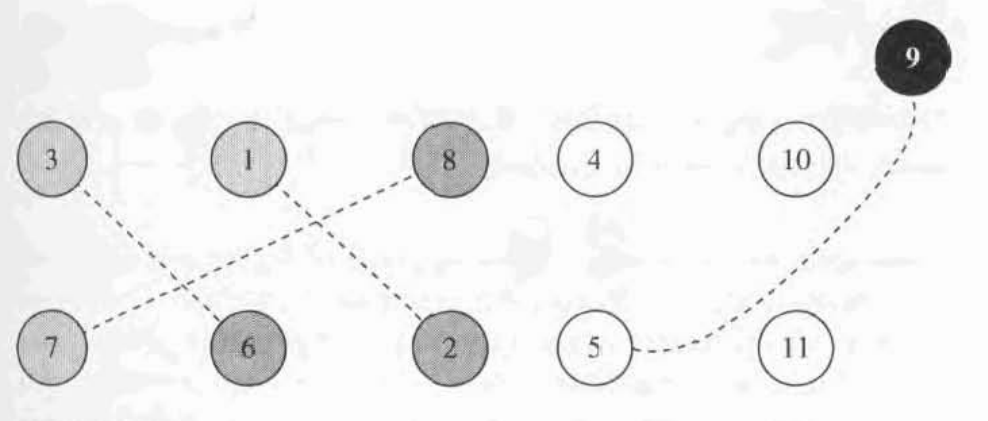
\includegraphics[width=0.4\textwidth]{Conflict_graphs_for_the_mtlltiplier_and_ALU_types}
    \caption{Conflict graphs for the multiplier and ALU types. \cite{main}}
    \label{Conflict_graphs_for_the_mtlltiplier_and_ALU_types}
\end{figure}

The execution delay for each operation is $\{[t_{i}, t_{i} + d_{i} - 1 ]; i + 1, 2, ...,n_{ops}$ and the edges of the conflict graph denote intersections among intervals, hence they are in an interval graph \cite{main}. Means that, in polynomial time, by applying interval sequence graph, it is much easier for designer to find the minimum number of colour used. Back to our circuit model in ``Fig. \ref{scheduled_sequencing_graph}", interval conflict graph can be obtained as shown in ``Fig. \ref{Intervals_corresponding_to_the_conflict_grap}".

\begin{figure}[h]
    \centering
    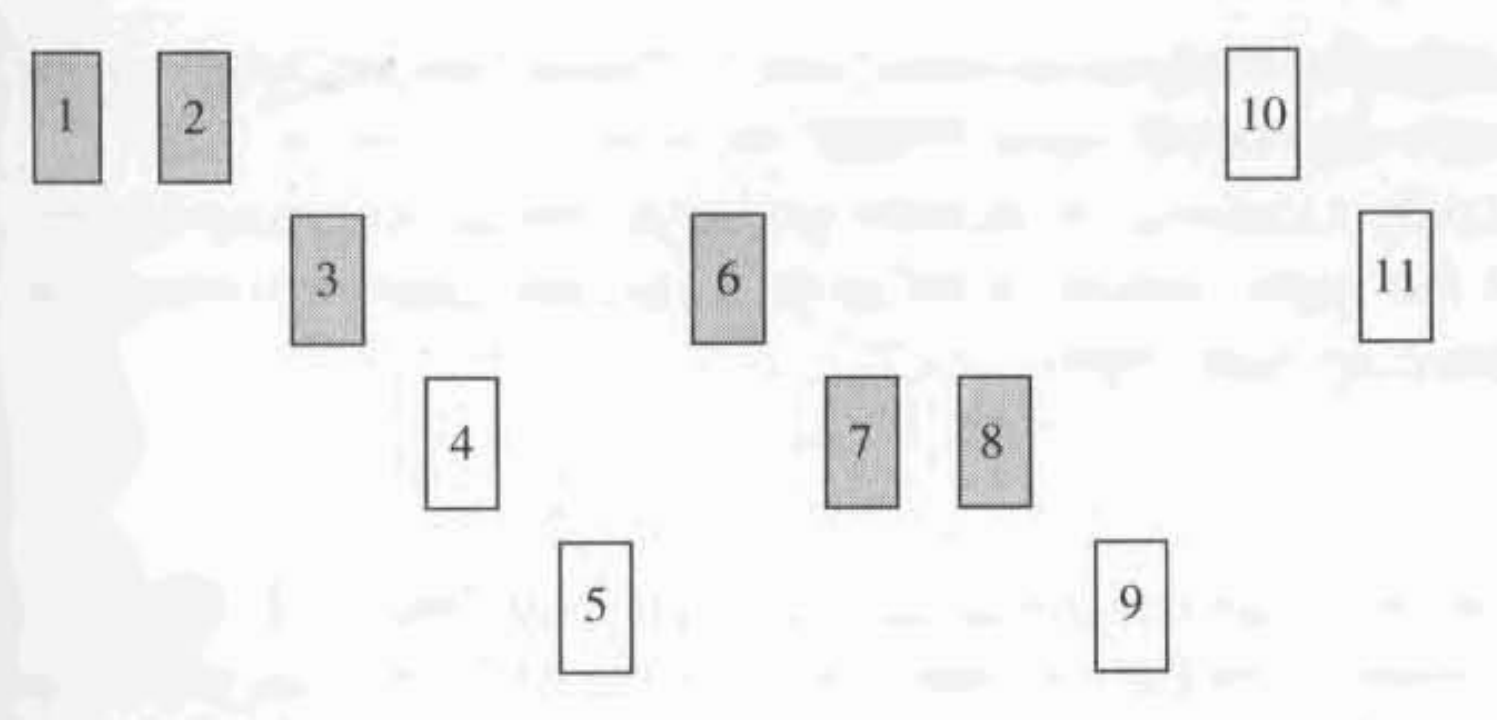
\includegraphics[width=0.4\textwidth]{Intervals_corresponding_to_the_conflict_graph}
    \caption{Intervals corresponding to the conflict graph. \cite{main}}
    \label{Intervals_corresponding_to_the_conflict_grap}
\end{figure}

In the next subtopic, we will discuss the method used to solve the binding problem for a given schedule and resource bound.


\subsection{ ILP model}

Binding problem for  circuit model whose specification include schedule and resource bound can be solved using ILP model \cite{main}. For the ILP model We use a set of binary decision variables with two indices, $ B=\{b_{ir};i=1,2,...,n_{pos};r=1,2,...,a\} $, and a set of binary decision constants with two indices, $ X=\{x_{il};i=1,2,...,n_{pos};l=1,2,...,\lambda+1\} $, where $ a\leq n_{ops} $ is an upper bound on the number of resources to be used, the binary variable,$ b_{ir} $ is 1 only when operation $ v_{i} $ is bound to resource r, i.e., $ \beta(v_{i})=(1,r) $ and the binary constant, $ x_{il} $ is 1 only when operation $ v_{i} $  starts in step 1 of the schedule, i.e., $ l = t{i} $ \cite{main}. 
Searching for a binding compatible with a given schedule (represented by $X$) and a resource bound $a$  is equivalent to searching for a set of values of B satisfying  the following constraints \cite{main}: 

\begin{equation}\label{a}
 \sum_{r=1}^{a} b_{ir} = 1, i=1,2,...,n_{ops} 
\end{equation}

\begin{equation}\label{b}
\sum_{i=1}^{n_{ops}} b_{ir}\sum_{m=l-d_{i}+1}^{l} x_{im} \leq 1, l=1,2,...,\lambda + 1, r=1,2,...,a 
\end{equation}

\begin{equation}\label{c}
b_{ir} \in \{0,1\}, 1 =1,2,...,n_{ops}, r=1,2,...,a
\end{equation}

 Based on our scheduled sequencing graph of ``Fig. \ref{scheduled_sequencing_graph}", the operations have two types and to make it simple we label multiplier with $1$ and ALU with $2$. So, a feasible binding satisfies the constraints \cite{main}: 

\begin{equation}\label{a}
 \sum_{r=1}^{a_{1}} b_{ir} = 1,\forall_{i} : \tau(v_{i})=1 
\end{equation}

\begin{equation}\label{b}
\sum_{i=:\tau(v_{i})=1}^{} b_{ir} x_{il} \leq 1, l=1,2,...,\lambda + 1, r=1,2,...,a_{1}
\end{equation}

\begin{equation}\label{c}
\sum_{r=1}^{a_{2}} b_{ir} = 1,\forall_{i} : \tau(v_{i})=2
\end{equation}

\begin{equation}\label{a}
 \sum_{i=:\tau(v_{i})=2}^{} b_{ir} x_{il} \leq 1, l=1,2,...,\lambda + 1, r=1,2,...,a_{2}
\end{equation}

The constants in the set X are all zero, except for $ x_{1,1},x_{1,1},x_{2,1},x_{3,2},x_{4,3},x_{5,4},x_{6,2},x_{7,3},x_{8,3},x_{9,4},x_{10,1},x_{11,2} $ which are 1. Then, an implementation with $ a_{1} =1$ multiplier would correspond to finding a solution to \cite{main} : 

\begin{equation}\label{b}
b_{i1} = 1, \forall_{i} \in \{1,2,3,6,7,8\}
\end{equation}

\begin{equation}\label{c}
\sum_{i\in \{1,2,3,6,7,8\}}^{} b_{i1} x_{il} \leq 1, l=1,2,...,5
\end{equation}


Such a solution does not exist, because the second constraint would imply $ b_{1,1}=b_{1,2} \leq 1 $, which contradicts the first one. An implementation with $ a_{1} =2$ multipliers would correspond to finding a solution to \cite{main}:


\begin{equation}\label{b}
 b_{i1}=b_{i2} = 1, \forall_{i} \in \{1,2,3,6,7,8\}
\end{equation}

\begin{equation}\label{c}
\sum_{i\in \{1,2,3,6,7,8\}}^{} b_{i1} x_{il} \leq 1, l=1,2,...,5
\end{equation}

\begin{equation}\label{c}
\sum_{i\in \{1,2,3,6,7,8\}}^{} b_{i2} x_{il} \leq 1, l=1,2,...,5
\end{equation}

which admits the solution $ b_{1,1}=1,b_{2,2}=1,b_{3,1}=1,b_{6,2}=1,b_{7,1}=1,b_{8,2}=1 $, all other elements of B with first subscript $ i \in \{I, 2,3.6,7,8\}$ being zero. The binding of the ALUs can be computed similarly. The list of binding is shown in ``Table \ref{tab1}" and can be illustrated using bound sequencing graph as shown in ``Fig. \ref{Scheduled_and_bound_sequencing}". The shaded area represent a resource and the operations within the shaded area are binded to the resource accordingly 


\begin{table}[htbp]
\caption{Binding result}
\begin{center}
\begin{tabular}{|c|c|c|c|}
\hline
$\beta(v_{1})$ & $(1,1)$  \\
$\beta(v_{2})$ &  $(1,2)$\\
$\beta(v_{3})$ &  $(1,1)$\\
$\beta(v_{4})$ &  $(2,1)$\\
$\beta(v_{5})$ &  $(2,1)$\\
$\beta(v_{6})$ &  $(1,2)$\\
$\beta(v_{7})$ &  $(1,1)$\\
$\beta(v_{8})$ &  $(1,2)$\\
$\beta(v_{9})$ &  $(2,2)$\\
$\beta(v_{10})$ &  $(2,1)$\\
$\beta(v_{11})$ &  $(2,1)$\\
\hline
\end{tabular}
\label{tab1}
\end{center}
\end{table}


\begin{figure}[h]
    \centering
    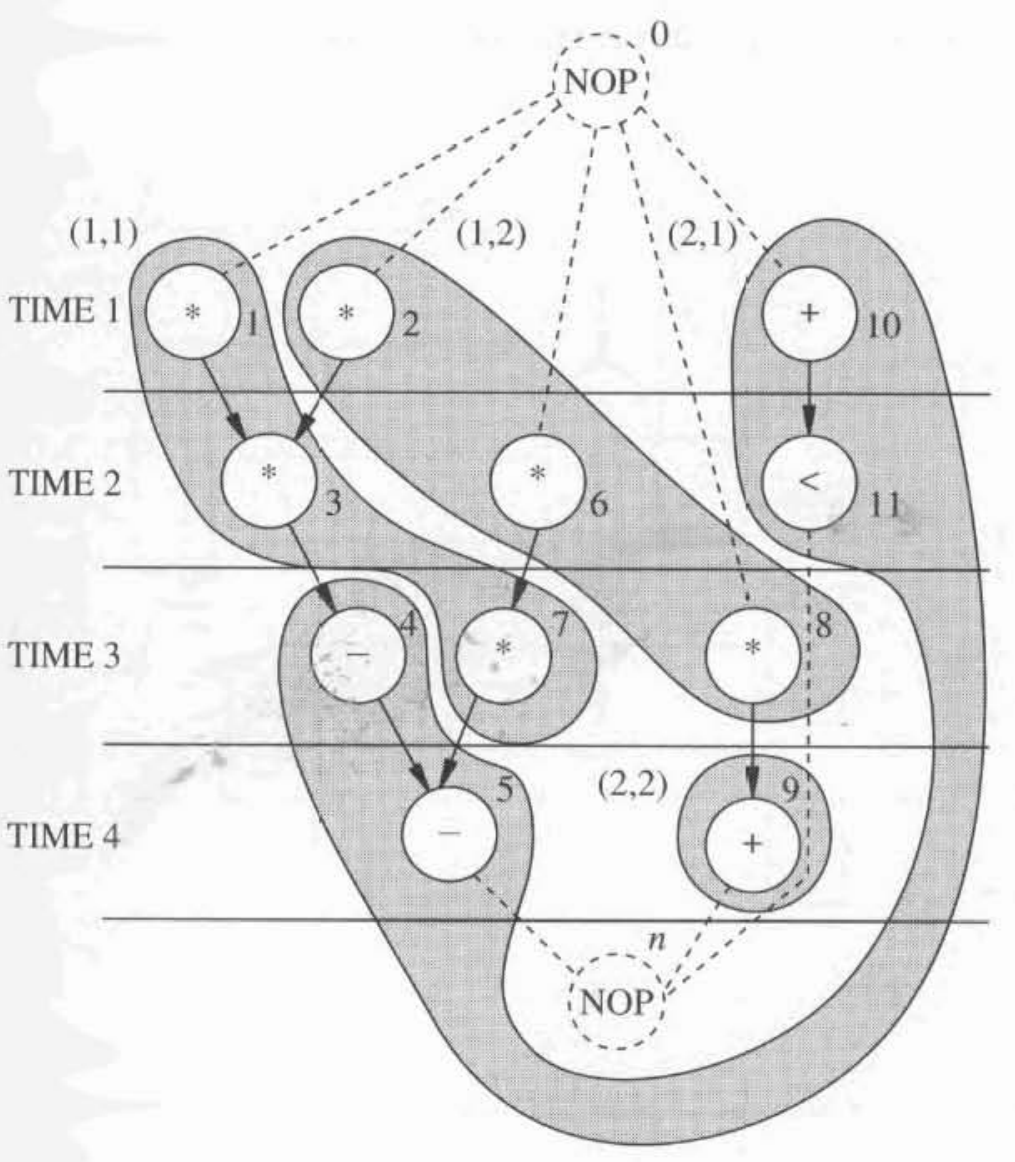
\includegraphics[width=0.4\textwidth]{Scheduled_and_bound_sequencing}
    \caption{Scheduled and bound sequencing. \cite{main}}
    \label{Scheduled_and_bound_sequencing}
\end{figure}


